\section{Elements of Web Search Engine}
	
\subsection{Crawler Module}
Web is huge and dynamic in nature as a result, all web search engines have a crawler module. This module contains the software that collects and categorizes the web's documents. The crawling software creates virtual robots, called spiders, that constantly crawls the Web gathering new information and webpages and returning to store them in a central repository.
	
\subsection{Page Repository}
The spiders return with new webpages, which are temporarily stored as complete webpages in the page repository. The new pages remain in the repository until they are sent to the indexing module, where their vital information is stripped to create a compressed version of the page.

\begin{figure}[h]
    \centering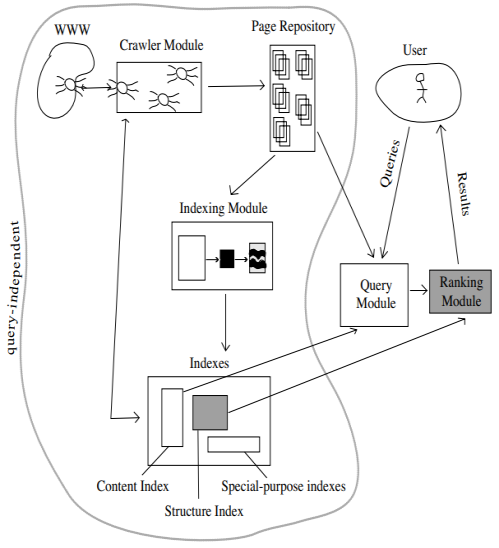
\includegraphics[scale=0.5]{engine.png}
    \caption{Elements of Web Search Engine}
    \label{fig:placeholder} % Unique label used for referencing the figure in-text
            %\addcontentsline{toc}{figure}{Figure \ref{fig:placeholder}} % Uncomment to add the figure to the table of contents
    \end{figure}

\subsection{Indexing Module}
The indexing module takes each new uncompressed page and extracts only the vital descriptors, creating a compressed description of the page that is stored in various indexes. The indexing module is like a black box function that takes the uncompressed page as input and outputs a “Cliffnotes” version of the page. The uncompressed page is then tossed out. We will be concentrating in PageRank index in this module.

\subsection{Indexes}
The indexes hold the valuable compressed information for each webpage. The first is called the content index. Here the content, such as keyword, title, and anchor text for each webpage, is stored in a compressed form using an inverted file structure. The crawler module sometimes accesses the structure index to find uncrawled pages. information regarding the hyperlink structure of pages in the search engine's index is gleaned during the indexing phase. This link information is stored in compressed form in the structure index. Special-purpose indexes are the final type of index. For example, indexes such as the image index and pdf index hold information that is useful for particular query tasks.\\
\\
The four modules above (crawler, page repository, indexers, indexes) and their corresponding data files exist and operate independent of users and their queries. Spiders are constantly crawling the Web, bringing back new and updated pages to be indexed and stored. These modules are circled and labeled as query-independent. Unlike the preceding modules, the query module is query-dependent and is initiated when a user enters a query, to which the search engine must respond in real-time.

\subsection{Query Module}
The query module converts a user's natural language query into a language that the search system can understand (usually numbers), and consults the various indexes in order to answer the query. For example, the query module consults the content index and its inverted file to find which pages use the query terms. These pages are called the relevant pages. Then the query module passes the set of relevant pages to the ranking module.

\subsection{Ranking Module}
The ranking module takes the set of relevant pages and ranks them according to some criterion. The outcome is an ordered list of webpages such that the pages near the top of the list are most likely to be what the user desires. The ranking module is perhaps the most important component of the search process because the output of the query module often results in too many relevant pages that the user must sort through. The set of relevant pages resulting from the query module is then presented to the user in order of their overall scores.